\chapter{Testing}

\section{Test strutturale}

\subsection{\texttt{creaOrdine()}}

\paragraph{Codice Java}

\inputminted[breaklines,tabsize=4,linenos]{java}{chapters/testing_white_box/creaOrdine.java}

\vfill

\pagebreak

\paragraph{Control Flow Graph}\mbox{}\newline

\noindent\begin{minipage}[t]{0.58\linewidth}
	\vspace{0pt}
	Il numero di cammini linearmente indipendenti è detto \emph{numero ciclomatico} di McCabe, e può essere calcolato equivalentemente in uno dei modi seguenti. Sia $G$ il grafo della funzione, allora risulta:
	\begin{enumerate}
		\item $V(G) = E - N + 2$ in cui $E = \text{\#archi in } G$, $N = \text{\#nodi in } G$
		\item $V(G) = P + 1$ con $P = \text{\#predicati in } G$
		\item $V(G) = R + 1$ con $R = \text{\#regioni chiuse in } G$
	\end{enumerate}%
	Nel nostro caso:%
	\begin{itemize}
		\item $E = 16$
		\item $N = 12$
		\item $P = 5$
		\item $R = 5$
	\end{itemize}%
	\begin{enumerate}
		\item $V(G) = E - N + 2 = 16 - 12 + 2 = 6$
		\item $P + 1 = 5 + 1 = 6$
		\item $R + 1 = 5 + 1 = 6$
	\end{enumerate}%
	\noindent I cammini di base sono:
	\begin{enumerate}
		\item 0-1
		\item 0-2
		\item 0-2-3-4-9-11
		\item 0-2-3-4-9-10-11
		\item 0-2-3-4-5-6-8-4-9-11
		\item 0-2-3-4-5-6-7-8-4-9-10-11
	\end{enumerate}
\end{minipage}
\hfill
\noindent\begin{minipage}[t]{0.38\linewidth}
	\vspace{0pt}
	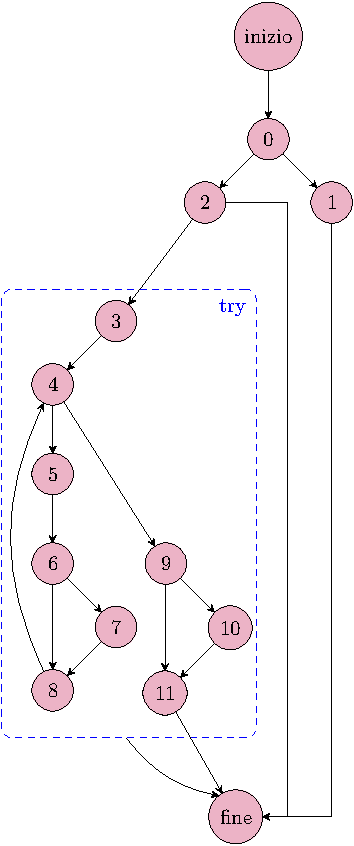
\includegraphics{chapters/testing_white_box/cfg_creaOrdine.pdf}
\end{minipage}

\vfill
\pagebreak

\paragraph{Test suite strutturale}\mbox{}\newline

\begin{table}[!hbp]
	\centering
	\begin{scenery}{colspec=lX}
		Caso d'uso: & CreaOrdine \\
		Attore primario & Cliente \\
		Attore secondario & - \\
		Descrizione & Un cliente genera un ordine contenente farmaci presenti in catalogo \\
		Pre-condizioni & Il cliente è autenticato \\
		{Sequenza di eventi \\ principale} &
			\begin{enumerate}
				\item Il cliente richiede al sistema di creare un ordine
				\item Il sistema mostra a video la lista dei farmaci
				\item Finché il cliente vuole aggiungere farmaci all'ordine
				\begin{enumerate}[label*=\arabic*.]
					\item Se viene richiesto un farmaco non da banco, il sistema chiede conferma del possesso della prescrizione
					\item Il cliente seleziona la quantità di farmaco desiderata
					\item Il sistema verifica che le scorte siano sufficienti
					\item Il sistema crea l'ordine con i farmaci inseriti e aggiorna le scorte
					\item \textit{punto di estensione}: GeneraOrdineAcquisto
				\end{enumerate}
				\item Il sistema mostra al cliente il resoconto dell'ordine e l'importo totale
				\item Se il cliente conferma l'acquisto
				\begin{enumerate}[label*=\arabic*.]
					\item Il sistema restituisce una ricevuta al cliente
				\end{enumerate}
				\item Altrimenti
				\begin{enumerate}[label*=\arabic*.]
					\item Il sistema elimina l'ordine
				\end{enumerate}
			\end{enumerate} \\
		Post-condizioni & È stato correttamente generato un ordine \\
		Casi d'uso correlati & Nessuno \\
		{Sequenza di eventi \\ alternativa} &
			\begin{enumerate}
				\item Al punto 3.1, il sistema mostra un messaggio di errore se il cliente non è in possesso della prescrizione
				\begin{enumerate}[label*=\arabic*.]
					\item Il farmaco non viene aggiunto all'ordine, il caso d'uso prosegue al punto 3
				\end{enumerate}
				\item Al punto 3.3, il sistema rileva che le scorte non sono sufficienti
					\begin{enumerate}[label*=\arabic*.]
						\item Il farmaco viene rimosso dall'ordine
					\end{enumerate}
			\end{enumerate} \\
	\end{scenery}
\end{table}


\vfill
\pagebreak

\subsection{\texttt{modificaFarmaco()}}

\paragraph{Codice Java}

\inputminted[breaklines,tabsize=4,linenos]{java}{chapters/testing_white_box/modificaFarmaco.java}

\paragraph{Control Flow Graph}\mbox{}\newline

\noindent\begin{minipage}[t]{0.58\linewidth}
	\vspace{0pt}
	Il numero di cammini linearmente indipendenti è detto \emph{numero ciclomatico} di McCabe, e può essere calcolato equivalentemente in uno dei modi seguenti. Sia $G$ il grafo della funzione, allora risulta:
	\begin{enumerate}
		\item $V(G) = E - N + 2$ in cui $E = \text{\#archi in } G$, $N = \text{\#nodi in } G$
		\item $V(G) = P + 1$ con $P = \text{\#predicati in } G$
		\item $V(G) = R + 1$ con $R = \text{\#regioni chiuse in } G$
	\end{enumerate}%
	Nel nostro caso:%
	\begin{itemize}
		\item $E = 6$
		\item $N = 5$
		\item $P = 2$
		\item $R = 2$
	\end{itemize}%
	\begin{enumerate}
		\item $V(G) = E - N + 2 = 6 - 5 + 2 = 3$
		\item $P + 1 = 2 + 1 = 3$
		\item $R + 1 = 2 + 1 = 3$
	\end{enumerate}%
	\noindent I cammini di base sono:
	\begin{enumerate}
		\item 0-1
		\item 0-1-2-4-1
		\item 0-1-2-3-4-1
	\end{enumerate}
\end{minipage}
\hfill
\noindent\begin{minipage}[t]{0.38\linewidth}
	\vspace{0pt}
	\begin{tikzpicture}[
    node/.style={circle, minimum height=20pt,text centered, draw=black, fill=purple!30},
    try/.style={rectangle, rounded corners=5, dashed, inner sep=8pt, draw=blue},
    node distance=0.8cm,
    arrow/.style={->,>=stealth}
]
\node (start) [node] {inizio};
\node (0) [node, below=of start] {$0$};
\node (1) [node, below=of 0] {$1$};
\node (2) [node, below left=of 1] {$2$};
\node (3) [node, below left=of 2] {$3$};
\node (4) [node, below=1.5cm of 2] {$4$};
\node (fine) [node, below = 4cm of 1] {fine};
\node (try) [try, fit=(0) (1) (2) (3) (4)] {};
\node [anchor=north west, inner sep=5pt, text=blue] at (try.north west) {try};



\draw[arrow] (start) -- (0);
\draw[arrow] (0) -- (1);
\draw[arrow] (1) -- (2);
\draw[arrow] (2) -- (3);
\draw[arrow] (2) -- (4);
\draw[arrow] (2) -- (4);
\draw[arrow] (3) -- (4);
\draw[arrow] (4) to [bend right=10] (1);
\draw[arrow] (1) to [bend left=50] (fine);
\draw[arrow] (try) to [bend right=10] (fine) {};

\end{tikzpicture}
\end{minipage}

\vfill
\pagebreak

\paragraph{Test suite strutturale}\mbox{}\newline

\begin{table}[!hbp]
	\centering
	\footnotesize
	\begin{tblr}{
			colspec = lXXXXX,
			hlines, vlines,
			row{1} = {font=\bfseries},
			measure=vbox
		}
		{Test \\ Case \\ ID} & Descrizione & {Cammino \\ Coperto} & Pre-condizioni & Input & Esito \\
		1 & Il farmaco è presente nel DB ma non nella collection locale, che risulta vuota & 0-1 & Il farmaco è presente nel DB ma non nella collection locale & -- &
       	Cammino non percorribile: la collection locale è sempre sincronizzata con il DB \\
		2 & La collection locale ha un solo farmaco che non è quello da modificare & 0-1-2-4-1 & -- & -- & Cammino non percorribile: se il farmaco è presente nel DB, deve essere presente anche nella collection locale \\
		3 & Il farmaco esiste & 0-1-2-3-4-1 & Il farmaco esiste & {Nome: Plasil \\ Prezzo: 11.50 \euro \\ Scorte: 30 \\ Prescrizione: \texttt{True}} & Farmaco modificato \\
	\end{tblr}
\end{table}


\section{Test funzionale}
In questa sezione ci occupiamo di riportare i risultati dell'applicazione della test suite definita nel \hyperref[cap:piano_test_funzionale]{Capitolo 4: Piano di Test Funzionale} all'implementazione Java del progetto. Di seguito vengono quindi riportati gli esiti dell'esecuzione dei vari test case, in particolare non vengono mostrati quei casi di test basati esclusivamente sull'input validation, poiché la validazione del formato dei parametri di input viene effettuata completamente a livello \texttt{Boundary}. Tutti i test sono effettuati sul package \texttt{Controller}.

\subsection{RegistraCliente}

\begin{table}[!hb]
	\centering
	\footnotesize
	\begin{testsuite}{colspec = lXXXlXX}
		{Test \\ Case \\ ID} & Descrizione & Classi di Equivalenza Coperte & Pre-condizioni & Input & {Output \\ Attesi} & {Post-condizioni \\ Attese} & Esito\\
		1 & Tutti gli input validi & Nome, Cognome, Username, Password, Email, DataNascita validi & Il cliente non è ancora registrato nel sistema & {Nome: Mario \\ Cognome: Rossi \\ Username: mariorossi \\ Password: miapassword \\ Email: mario@gmail.com \\ DataNascita: 22-06-1989} & Registrazione effettuata & Il cliente è stato correttamente registrato nel sistema & PASS \\
		13 & Username già presente nel sistema & Username già esistente \texttt{[ERROR]}, Nome, Cognome, Password, DataNascita ed Email validi & Username ``pippo2002'' già presente nel sistema & {Nome: Pippo \\ Cognome: Baudo \\ Username: pippo2002 \\ Password: miapassword \\ Email: pippo@gmail.com \\ DataNascita: 1989-06-22} & {Username già \\ utilizzato} & -- & PASS \\
		14 & Email già presente nel sistema & Email già esistente \texttt{[ERROR]}, Nome, Cognome, Password, DataNascita e Username validi & Email ``pippo@gmail.com'' già presente nel sistema & {Nome: Pippo \\ Cognome: Baudo \\ Username: pippo2002 \\ Password: miapassword \\ Email: pippo@gmail.com \\ DataNascita: 1989-06-22} & {Email già \\ utilizzata} & -- & PASS \\
	\end{testsuite}
\end{table}

\subsection{LoginUtente}

\begin{table}[H]
	\centering
	\footnotesize
	\begin{testsuite}{colspec = lXXXXXX}
		{Test \\ Case \\ ID} & Descrizione & Classi di Equivalenza Coperte & Pre-condizioni & Input & {Output \\ Attesi} & {Post-condizioni \\ Attese} & Esito \\
		1 & Tutti gli input validi & Username, Password validi & {L'utente deve essere \\ correttamente \\ registrato nel sistema} & {Username: mariorossi \\ Password: miapassword} & Login effettuato & L'utente è entrato correttamente nel sistema & PASS\\
		6 & Password errata & Password errata \texttt{[ERROR]}, Username valido & L'utente esiste nel sistema e ha come password `passwd' & {Username: mariorossi \\ Password: ciao} & Password errata & -- & PASS\\
		7 & Username non registrato & Username non registrato \texttt{[ERROR]} & L'utente non esiste nel sistema & {Username: geronimo \\ Password: stilton} & Utente non registrato & -- & PASS\\
	\end{testsuite}
\end{table}

\subsection{AggiungiFarmaco}

\begin{table}[H]
	\centering
	\footnotesize
	\begin{testsuite}{colspec = lXXXlXX}
		{Test \\ Case \\ ID} & Descrizione & Classi di Equivalenza Coperte & Pre-condizioni & Input & {Output \\ Attesi} & {Post-condizioni \\ Attese} & Esito \\
		1 & Tutti gli input validi & Nome, Prezzo, Scorte e Prescrizione (sia \texttt{True} che \texttt{False}) validi & Il farmaco non è presente nel sistema & {Nome: Rocefin \\ Prezzo: 15.00 \euro \\ Scorte: 60 \\ Prescrizione: \texttt{boolean}} & Farmaco aggiunto & Il farmaco viene correttamente aggiunto al catalogo & PASS \\
		6 & Nome già memorizzato & Nome già memorizzato \texttt{[ERROR]}, Prezzo, Scorte e Prescrizione (sia \texttt{True} che \texttt{False}) validi & Esiste già un farmaco con il nome inserito & {Nome: Cistalgan \\ Prezzo: 19.90 \euro \\ Scorte: 50 \\ Prescrizione : \texttt{boolean}} & Farmaco già esistente & -- & PASS \\
	\end{testsuite}
\end{table}

\subsection{CercaFarmaco}

\begin{table}[H]
	\centering
	\footnotesize
	\begin{testsuite}{colspec = lXXXlXl}
		{Test \\ Case \\ ID} & Descrizione & Classi di Equivalenza Coperte & Pre-condizioni & Input & {Output \\ Attesi} & {Post-\\condizioni \\ Attese} & Esito \\
		1 & Nome del farmaco valido & Nome del farmaco valido & Il farmaco è presente nel catalogo & Nome: Tachipirina & Il farmaco viene mostrato a video & -- & PASS \\
		4 & Nome di un farmaco che non esiste & Nome di un farmaco che non esiste \texttt{[ERROR]} & Il farmaco con nome ``Tachipirina'' non esiste & Nome: Tachipirina & Il farmaco non esiste & -- & PASS \\
	\end{testsuite}
\end{table}

\subsection{EliminaFarmaco}

\begin{table}[H]
	\centering
	\footnotesize
	\begin{testsuite}{colspec = lXXXlXX}
		{Test \\ Case \\ ID} & Descrizione & Classi di Equivalenza Coperte & Pre-condizioni & Input & {Output \\ Attesi} & {Post-condizioni \\ Attese} & Esito \\
		1 & Nome del farmaco valido & Nome del farmaco valido & Il farmaco è presente nel catalogo & Nome: Tachipirina & Farmaco cancellato & Il farmaco viene cancellato dal catalogo & PASS \\
		4 & Il farmaco non esiste & Farmaco non presente nel sistema \texttt{[ERROR]} & Non esiste il farmaco chiamato ``Tachipirina'' & Nome: Tachipirina & Non puoi eliminare un farmaco che non esiste & -- & PASS \\
	\end{testsuite}
\end{table}

\subsection{ModificaFarmaco}

\begin{table}[H]
	\centering
	\footnotesize
	\begin{testsuite}{colspec = lXXXlXX}
		{Test \\ Case \\ ID} & Descrizione & Classi di Equivalenza Coperte & Pre-condizioni & Input & {Output \\ Attesi} & {Post-condizioni \\ Attese} & Esito \\
		1 & Tutti gli input validi, prescrizione \texttt{True} & Nome, Prezzo, Scorte e Prescrizione (\texttt{True}) validi & Il farmaco è presente nel sistema & {Nome: Tachipirina \\ Prezzo: 11.44 \euro \\ Scorte: 100 \\ Prescrizione: \texttt{True}} & {Modifica \\ effettuata} & Il farmaco viene correttamente modificato & PASS \\
		2 & Tutti gli input validi, prescrizione \texttt{False} & Nome, Prezzo, Scorte e Prescrizione (\texttt{False}) validi & Il farmaco è presente nel sistema & {Nome: Tachipirina \\ Prezzo: 11.44 \euro \\ Scorte: 100 \\ Prescrizione: \texttt{False}} & {Modifica \\ effettuata} & Il farmaco viene correttamente modificato & PASS \\
		7 & Il nome del farmaco non esiste & Nome non presente nel sistema \texttt{[ERROR]}, Prezzo, Scorte e Prescrizione validi & Il farmaco ``Tachipirina'' non esiste nel sistema & {Nome: Tachipirina \\ Prezzo: 11.44 \euro \\ Scorte: 100 \\ Prescrizione: \texttt{False}} & Il farmaco non esiste & -- & PASS \\
	\end{testsuite}
\end{table}

\subsection{GeneraReport}

\begin{table}[H]
	\centering
	\footnotesize
	\begin{testsuite}{colspec = llXXX}
		{Test \\ Case \\ ID} & Descrizione & {Classi di Equivalenza \\ Coperte} & Input & Output Attesi & Esito \\
		1 & {Tutti gli input \\ validi} & DataInizio, DataFine validi & {DataInizio: 01-06-2024 \\ DataFine: 31-06-2024} & Il report viene generato & PASS \\
	\end{testsuite}
\end{table}

\subsection{GeneraOrdineAcquistoFarmacista}

\begin{table}[!hbp]
	\centering
	\footnotesize
	\begin{testsuite}{colspec = lXXXlXX}
		{Test \\ Case \\ ID} & Descrizione & Classi di Equivalenza Coperte & Pre-condizioni & Input & {Output \\ Attesi} & {Post-condizioni \\ Attese} & Esito \\
		1 & Ordine valido & Farmaci-Quantità valido & Esistono nel sistema i farmaci 'Tachipirina' e 'Fluifort' & {[('Tachipirina', 5),\\ ('Fluifort', 10)]} & Ordine di acquisto generato & Un ordine di acquisto viene correttamente creato & PASS \\
		2 & Ordine vuoto & Lista vuota \texttt{[ERROR]} & -- & -- & Non puoi creare un ordine di acquisto vuoto & -- & PASS \\
	\end{testsuite}
\end{table}

\subsection{RitiraOrdine}

\begin{table}[!hb]
	\centering
	\footnotesize
	\begin{testsuite}{colspec = lXXXXXX}
		{Test \\ Case \\ ID} & Descrizione & Classi di Equivalenza Coperte & Pre-condizioni & Input & {Output \\ Attesi} & {Post-condizioni \\ Attese} & Esito \\
		1 & Id dell'ordine valido & Id dell'ordine valido & -- & Id: 5ea930bc-f0a5-427a-8ca1-f9a2a6146948 & Stato ordine cambiato con successo & Lo stato dell'ordine è stato cambiato con successo & PASS \\
		4 & Id inesistente & Id inesistente \texttt{[ERROR]} & Non esiste un farmaco con id ``5ea930bc-f0a5-427a-8ca1-f9a2a6146948'' & Id: 5ea930bc-f0a5-427a-8ca1-f9a2a6146948 & L'ordine non esiste & -- & PASS \\
	\end{testsuite}
\end{table}

\subsection{RegistraConsegnaOrdineAcquisto}

\begin{table}[H]
	\centering
	\footnotesize
	\begin{testsuite}{colspec = lXXXXXX}
		{Test \\ Case \\ ID} & Descrizione & Classi di Equivalenza Coperte & Pre-condizioni & Input & {Output \\ Attesi} & {Post-condizioni \\ Attese} & Esito \\
		1 & Id dell'ordine di acquisto valido & Id dell'ordine di acquisto valido & -- & {Id: 5ea930bc-f0a5-427a-8ca1-f9a2a6146948} & Ordine ricevuto & Lo stato dell'ordine di acquisto e le scorte in magazzino sono aggiornati & PASS \\
		4 & Id inesistente & Id inesistente \texttt{[ERROR]} & Non esiste un ordine di acquisto con Id ``5ea930bc-f0a5-427a-8ca1-f9a2a6146948'' & Id: 5ea930bc-f0a5-427a-8ca1-f9a2a6146948 & L'ordine di acquisto non esiste & -- & PASS \\
	\end{testsuite}
\end{table}

\subsection{CreaOrdine}

\begin{table}[!hbp]
	\centering
	\footnotesize
	\begin{testsuite}{colspec = lXXXlXX}
		{Test \\ Case \\ ID} & Descrizione & Classi di Equivalenza Coperte & Pre-condizioni & Input & {Output \\ Attesi} & {Post-condizioni \\ Attese} & Esito \\
		1 & Ordine valido, l'ordine non esaurisce le scorte di nessun farmaco & Farmaci-Quantità valido & Esistono nel sistema i farmaci 'Tachipirina' e 'Fluifort' con scorte rispettivamente di 80 e 120 & {[('Tachipirina', 5),\\ ('Fluifort', 10)]} & Ordine generato & Ordine creato: scorte in magazzino decrementate & PASS \\
		2 & Ordine valido, l'ordine esaurisce le scorte di un farmaco & Farmaci-Quantità valido & Esistono nel sistema i farmaci 'Tachipirina' e 'Fluifort' con scorte rispettivamente di 80 e 120 & {[('Tachipirina', 80),\\ ('Fluifort', 10)]} & Ordine generato & Ordine creato. Le scorte in magazzino vengono correttamente decrementate e viene generato un ordine di fornitura per il farmaco esaurito, richiedendone una quantità di default & PASS \\
		3 & Ordine vuoto & Lista vuota \texttt{[ERROR]} & -- & -- & Non puoi creare un ordine vuoto & -- & PASS \\
		4 & Ordine invalido per scorte insufficienti & Scorte insufficienti \texttt{[ERROR]} & Esistono nel sistema i farmaci 'Tachipirina' e 'Fluifort' con scorte rispettivamente di 80 e 120 & {[('Tachipirina', 5),\\ ('Fluifort', 150)]} & Ordine non creato per scorte insufficienti & -- & PASS \\
	\end{testsuite}
\end{table}
